\chapter{Related Work and the Problem This Thesis Addresses}
\label{ch:related}

The counting problem in this thesis sits at the junction of three older lines of work. The first is instance segmentation: the assignment of a separate mask to every object, rather than a single label per pixel. The second is visual counting, which began with crowds and cells and has only recently been asked to count goods that hide one another. The third is computational color constancy, the attempt to separate the color of a surface from the color of the light that falls on it. A brewery aisle forces all three to be solved together, on a moving forklift, from a camera that sees only one face of the stack. This chapter sets out the principles, then the systems that have already been built for warehouses and cartons, and then the precise gap that the rest of the thesis fills.

\section{Principles of segmentation, counting, and color}
\label{sec:principles}

\subsection{What the camera records}
\label{sec:formation}

A digital camera does not record the paint on a crate. It records a number in each of three channels, and that number mixes the spectrum of the lamp, the reflectance of the plastic, the spectral sensitivity of the sensor, and the exposure chosen by the shutter. Under the standard simplification used throughout color constancy, a Lambertian surface under a single illuminant collapses to a diagonal model~\cite{gijsenij2011survey}. If $\mathbf{R}(x)\in\mathbb{R}^{3}$ is the reflectance of the surface at pixel $x$ and $\mathbf{L}\in\mathbb{R}^{3}$ is a positive illuminant vector, the observed intensity is the element-wise product
\begin{equation}
\mathbf{I}(x) = \mathbf{L} \odot \mathbf{R}(x).
\label{eq:diagonal}
\end{equation}
The same crate, moved from a north-facing door to a sodium lamp deeper in the aisle, changes $\mathbf{L}$ and therefore changes $\mathbf{I}$, while $\mathbf{R}$ stays fixed. Any classifier that memorizes $\mathbf{I}$ is memorizing the lamp as well as the plastic.

Three further effects sit on top of~\eqref{eq:diagonal} in the scene of this thesis, and none of them is a small correction. Shading from the forks and from the crate above multiplies $\mathbf{I}$ by a scalar that varies smoothly across the face. A neighboring crate of another color leaks into the mask wherever the predicted boundary is a few pixels too wide. Motion of the forklift, if the shutter is open for more than a few milliseconds, smears the horizontal lip of each crate along the direction of travel. The diagonal model remains the right first equation because the two updates in Chapter~\ref{ch:methods} attack illuminant and geometry separately, but the estimate in Chapter~\ref{ch:system} puts shading, edge mixing, and a detection loss that grows with blur back into the observation model so that the diagonal story is not asked to carry the whole scene.

The geometry of the same image is a projective map~\cite{hartley2004mvg}. A pinhole camera sends a point $\mathbf{X}$ on the front face of the stack to a pixel
\begin{equation}
s \begin{bmatrix} u \\ v \\ 1 \end{bmatrix}
= K \,[\,R \mid \mathbf{t}\,]\,
\begin{bmatrix} \mathbf{X} \\ 1 \end{bmatrix},
\label{eq:pinhole}
\end{equation}
with $K$ the intrinsics, $R$ and $\mathbf{t}$ the pose of the camera relative to the face, and $s$ a scale. When the front face is approximately a plane, the map from that plane to the image is a homography. Calibration of $K$ by a planar target~\cite{zhang2000calibration} and estimation of the homography are therefore sufficient to put detections into metres on the crate face. That metric plane is what the lattice counter of Chapter~\ref{ch:methods} assumes. It is not a reconstruction of the whole pallet in three dimensions.

\subsection{Detection, semantic segmentation, and instance segmentation}
\label{sec:tasks}

Object detection returns a box and a class. The modern two-stage line begins with region proposals and a convolutional classifier~\cite{girshick2014rcnn}, speeds the classifier by sharing the feature map~\cite{girshick2015fastrcnn}, and then learns the proposals themselves~\cite{ren2015faster}. A cascade of detectors trained at increasing intersection-over-union tightens the boxes that survive~\cite{cai2018cascade}. One-stage detectors skip the proposal stage. SSD places default boxes on several feature maps~\cite{liu2016ssd}. RetinaNet shows that the extreme imbalance between background anchors and object anchors can be handled by a focal loss that down-weights the easy negatives~\cite{lin2017focal}. FCOS removes anchors and regresses a box from each foreground pixel~\cite{tian2019fcos}. CornerNet detects a pair of corners and groups them~\cite{law2018cornernet}. CenterNet detects the center point and reads the box size from that point~\cite{zhou2019centernet}. YOLO, from its first version, frames detection as one regression on a grid~\cite{redmon2016yolo}.

Semantic segmentation assigns a class to every pixel and does not say which crate is which. Fully convolutional networks showed that a classifier can be turned into a dense predictor~\cite{long2015fcn}. U-Net added a skip-connected decoder that restores spatial detail~\cite{ronneberger2015unet}. DeepLabv3+ combined atrous convolution in the encoder with a light decoder~\cite{chen2018deeplab}. None of these outputs can be counted by connected components when two crates of the same color touch, because the two crates are one component.

Instance segmentation returns a separate mask per object. Mask R-CNN adds a small fully convolutional mask head on each region of interest of Faster R-CNN, and aligns the pooled features with the box by bilinear sampling~\cite{he2017maskrcnn}. The mask head is class-specific in the original design: the network predicts a mask for every class and the box class selects which mask is kept. That separation matters for the brewery. Color type and spatial extent are different questions. A mask can be right while the color name is wrong, and the counting stage should be able to use the mask either way.

The optimization and generalization background used throughout is the standard one for deep networks~\cite{goodfellow2016dl,lecun2015nature}. Training these models depends on large labeled sets. Pascal VOC established the detection challenge that the first deep detectors were measured on~\cite{everingham2010pascal}. ImageNet supplied the pretraining that made those detectors converge~\cite{deng2009imagenet}. COCO raised the instance count per image and became the standard mask benchmark~\cite{lin2014coco}. A warehouse of identical crates is a different distribution from COCO. The features transfer; the decision threshold and the color head do not, which is why a prototype head trained on crate colors is part of the update rather than a reuse of the COCO classifier.

\subsection{The one-stage mask and the YOLO line}
\label{sec:yolo}

Two-stage mask heads are accurate and, for a forklift that may clear the camera in under a second, often too sequential. YOLACT removed the region-wise mask head. It predicts a dictionary of prototype masks on the whole image and a vector of coefficients on each detection, then forms the instance mask as a linear combination of the prototypes, cropped to the box~\cite{bolya2019yolact}. YOLACT++ keeps that assembly and improves the prototypes and the backbone~\cite{bolya2022yolactpp}. The assembly is
\begin{equation}
M = \sigma\!\left( P\, c \right),
\label{eq:yolact}
\end{equation}
where $P$ is the stack of prototype masks, $c$ is the coefficient vector of one detection, and $\sigma$ is a sigmoid. The prototypes are shared. Individuality lives in $c$. FastSAM later showed that a YOLOv8 segmenter, which uses this same assembly, can be trained as a fast proposal generator for a segment-anything style task~\cite{zhao2023fastsam}.

Other one-stage designs are worth keeping in view because they expose different failure modes. SOLO predicts a mask on a spatial grid, so that location itself is the identity of the instance~\cite{wang2020solo}. SOLOv2 makes the mask weights dynamic and adds a matrix non-maximum suppression that is cheaper than a pixel-wise suppression~\cite{wang2020solov2}. CondInst generates the weights of a tiny mask head from the instance features, conditioned on the instance~\cite{tian2020condinst}. BlendMask combines a top-down attention on a bottom-up position-sensitive map~\cite{chen2020blendmask}. PolarMask represents the contour as rays from the center, which is attractive for compact blobs and brittle for a crate whose visible region is a rectangle with a bite taken out by occlusion~\cite{xie2020polarmask}. SparseInst activates a sparse set of instance queries and avoids non-maximum suppression~\cite{cheng2022sparseinst}. BoxInst shows that a projection loss and a pairwise color affinity can train a CondInst-style mask from boxes alone~\cite{tian2021boxinst}. The pairwise term is relevant here: plastic crates are nearly constant in color inside the face, so a color-affinity prior agrees with the object, and it also agrees with the failure mode in which two adjacent crates of the same color are glued into one mask.

The YOLO family itself is the practical backbone of the baseline used in this thesis. After the original grid regression~\cite{redmon2016yolo}, YOLO9000 introduced joint training and anchor boxes~\cite{redmon2017yolo9000}, and YOLOv3 moved to a feature pyramid and a stronger backbone~\cite{redmon2018yolov3}. YOLOv4 organized a large set of training and architecture choices that had been scattered across papers~\cite{bochkovskiy2020yolov4}. YOLOv5 made that line reproducible as a maintained implementation~\cite{jocher2020yolov5}. YOLOv6 reworked the neck and the loss for industrial deployment~\cite{li2022yolov6}. YOLOX replaced the coupled head and the anchors with a decoupled head and an anchor-free assignment~\cite{ge2021yolox}. YOLOv7 studied which of the so-called freebies survive re-parameterization and set a high bar for real-time detection~\cite{wang2023yolov7}. YOLOv8, released as software rather than as a single paper, is the version whose segmentation head follows~\eqref{eq:yolact} and whose detection head is decoupled~\cite{jocher2023yolov8}. YOLOv9 introduced programmable gradient information so that the loss sees a more complete view of the input, and showed a gain on the mask task as well as on boxes~\cite{wang2024yolov9}. YOLOv10 removed the need for non-maximum suppression by a consistent dual assignment~\cite{wang2024yolov10}. YOLO11 continues the same implementation line~\cite{jocher2024yolo11}. Real-time transformer detectors, from DETR~\cite{carion2020detr} through deformable attention~\cite{zhu2021deformable} and denoising queries~\cite{zhang2023dino} to RT-DETR~\cite{zhao2024rtdetr}, have closed the speed gap. They are not the baseline here, because the crate system needs a mask, a stable box center, and a small extra head, and the YOLACT-style segmenter already provides the first two.

The feature pyramid that these detectors share is the structure of Lin and colleagues~\cite{lin2017fpn}: a top-down path that carries semantics down to high-resolution maps, and lateral connections that restore detail. EfficientDet replaced the plain sum of those laterals with a weighted bidirectional pyramid~\cite{tan2020efficientdet}. CSPNet reduced duplicate gradient flow by splitting the feature map, and that split is the ancestor of the cross-stage modules in the later YOLO backbones~\cite{wang2020cspnet}. Channel attention of the squeeze-and-excitation kind~\cite{hu2018senet}, the convolutional block attention module~\cite{woo2018cbam}, and coordinate attention~\cite{hou2021coordatt} are the usual tools when a designer wants the network to prefer one spatial axis. The vertical-feature neck of YOLO-vf-seg, defined properly in Section~\ref{sec:problem-gap}, is a deliberate use of that last idea: on a side view the informative edges are horizontal, so the neck should be allowed to treat the vertical coordinate differently from the horizontal one.

Backbones have their own literature, and the warehouse papers cited in the next section borrow from it. Residual networks made the depth of the backbone a free parameter rather than an optimization accident~\cite{he2016resnet}. MobileNet and MobileNetV2 showed that depthwise separable convolution and inverted residuals keep accuracy when the computer is small~\cite{howard2017mobilenet,sandler2018mobilenetv2}. EfficientNet scaled depth, width, and resolution together~\cite{tan2019efficientnet}. ConvNeXt modernized a plain convolutional network with the training recipe of transformers~\cite{liu2022convnext}. The vision transformer and the Swin transformer replaced the sliding window with attention over patches~\cite{dosovitskiy2021vit,liu2021swin}, using the attention mechanism introduced for sequence transduction~\cite{vaswani2017attention}. RepVGG trains a multi-branch block and folds it into a single convolution at inference~\cite{ding2021repvgg}. That fold is why several recent warehouse models can quote a high frame rate after having trained a heavier block. The present design does not replace the backbone. It adds a color head whose parameter count is a fraction of one percent of a medium segmenter, and a counting stage that is not a network at all.

Box regression losses affect whether two stacked crates receive two centers or one merged box. Generalized IoU adds the empty area of the smallest enclosing box to the ordinary overlap penalty~\cite{rezatofighi2019giou}. Distance-IoU and the complete-IoU variant add the distance between centers and the aspect ratio, so that a non-overlapping prediction still receives a gradient~\cite{zheng2020diou}. Wise-IoU modulates that geometry by a focusing coefficient that depends on how the rest of the batch is behaving~\cite{tong2023wiou}. IoU-Net argued that the classification score is a poor proxy for localization quality and predicted the overlap directly~\cite{jiang2018iounet}. Generalized focal loss and VarifocalNet fold a localization quality into the classification target so that non-maximum suppression ranks boxes by a score that means what the suppression thinks it means~\cite{li2020gfl,zhang2021vfnet}. For crates, a high classification score on a box that straddles two stacked faces is exactly the error that produces a missed count. The lattice stage can repair some of those misses. It cannot repair them if the center it receives lies between two true cells.

Mask losses have a similar tension between region overlap and boundary fidelity. The Dice coefficient~\cite{dice1945} and its soft version in V-Net~\cite{milletari2016vnet} emphasize overlap and are stable when the crate occupies a modest part of the window. A generalized Dice reweights classes by the inverse of their volume~\cite{sudre2017gdice}. Overlap losses under-penalize a boundary that is off by a few pixels, and a few pixels on a crate lip are the difference between one instance and two. PointRend treats the uncertain boundary pixels as a rendering problem and classifies them at higher resolution~\cite{kirillov2020pointrend}. Boundary patch refinement crops small windows along the predicted contour and re-segments those windows~\cite{tang2021bpr}. Both are compatible with YOLO-vf-seg as a later refinement. They are not the updates proposed here, because the dominant counting errors in a regular stack are missed cells and wrong colors, not a contour that is cosmetically rough.

\subsection{Counting what is visible and what is hidden}
\label{sec:counting-principles}

The oldest learned counter regresses a density map whose integral is the count. Lempitsky and Zisserman introduced that idea so that a model could be trained from dotted annotations~\cite{lempitsky2010count}. A multi-column network estimates the density at several receptive fields when the objects vary in scale~\cite{zhang2016mcnn}. CSRNet keeps a single deeper column and uses dilated convolution to enlarge the field without losing resolution~\cite{li2018csrnet}. Later losses match the predicted and target distributions rather than only their pixel values, which reduces the tendency to place a blurry mass where a sharp peak should be~\cite{wang2020dmcount}. A composition loss combines counting, density, and localization~\cite{idrees2018composition}. Counting in the wild showed that the same idea extends past crowds when the annotations are still points~\cite{arteta2016counting}.

A density map is the wrong intermediate for typed crates. The integral of a density does not remember which color produced which mass of the integral, and a side view of a stack violates the assumption that every object contributes a visible dot. The bottom row is partly behind the forks. Crates in the second and third rank of the pallet are not in the image at all. Integrating a density over the visible face estimates the visible count, and only under the further assumption that occlusion eats a similar fraction of every crate. That assumption is false at the bottom and at the top of the frame.

Detection counting is the other extreme. Each surviving mask contributes one to a tally. It is simple, it preserves class, and it is biased low by every miss. Area-ratio counting, discussed with the warehouse systems in the next section, tries to recover partial crates by dividing a visible area by a nominal area. It recovers a fraction of a crate and then has to round. Geometry-aware counting uses the fact that the objects are the same size. That is the opening this thesis uses. The front face of a beer-crate stack is a lattice with known pitch. A missed detection is often a hole in an otherwise regular grid, and a hole with supported neighbors is a different event from an empty region of the aisle.

Hidden objects can also be counted from volume. Dumery and colleagues decompose the count of identical stacked objects into a reconstructed volume times an occupancy ratio estimated from a depth map, and they show that people are poor at the same task~\cite{dumery2024stacked}. Their method assumes a container seen from several views, objects that are approximately identical, and a depth estimator. A brewery forklift presents a different bargain. The objects are identical only within a color, the colors matter, the useful view is the side rather than the top, and the hidden dimension is a small integer: how many crates deep the pallet is. Multiplying an occupied front lattice by that integer is a coarser, and for this scene a more direct, use of the same idea that hidden extent should be measured rather than hallucinated pixel by pixel.

Associative embedding groups detections that belong to the same structured object by a learned tag~\cite{newell2017ae}. A Hungarian assignment matches two sets at minimum cost~\cite{kuhn1955hungarian}. PLC does not need either construction for the front face, because the lattice supplies the grouping. Both remain relevant if a later version of the system has to associate the same physical crate across a long passage with a moving camera. The estimate in this thesis uses a simpler rule, and Chapter~\ref{ch:system} reports that the simpler temporal rule over-counts.

\subsection{Color constancy, and why a uniform face breaks it}
\label{sec:color-principles}

Color constancy estimates $\mathbf{L}$ in~\eqref{eq:diagonal} so that a corrected image $\mathbf{I}(x)\oslash\hat{\mathbf{L}}$ depends on reflectance. The gray-world hypothesis says that the average reflectance in the scene is gray, so the average of $\mathbf{I}$ is a sufficient estimate of the illuminant~\cite{buchsbaum1980grayworld}. The Minkowski family generalizes that average. With $p\ge 1$,
\begin{equation}
\hat{\ell}_c
= \left(
\frac{1}{\lvert\Omega\rvert}
\sum_{x\in\Omega} \lvert I_c(x)\rvert^{p}
\right)^{1/p}.
\label{eq:minkowski}
\end{equation}
The case $p=1$ is gray-world. The case $p\to\infty$ is max-RGB, the channel-wise maximum. Shades-of-gray argues that a moderate $p$, commonly six, is a better default across photographs than either extreme~\cite{finlayson2004shades}. Edge-based variants apply the same norms to image derivatives so that large flat surfaces, which dominate a gray-world average and carry little information about the illuminant, do not drown the estimate~\cite{vandeweijer2007edge}. Retinex theory is the perceptual ancestor of these algorithms: lightness is inferred from spatial comparisons rather than from the absolute intensity at a point~\cite{land1971retinex}.

Learned estimators replace the norm. Oh and Kim cast illuminant estimation as classification over a discrete set of lights~\cite{oh2017colorclass}. FC4 predicts a local illuminant and a confidence at every patch and pools them with the confidence as a weight, precisely because many patches are consistent with almost any lamp~\cite{hu2017fc4}. Fast Fourier color constancy reduces illuminant estimation to localization on a torus and runs fast enough for a camera pipeline~\cite{barron2017ffcc}. The survey of Gijsenij, Gevers, and van de Weijer remains the right map of the assumptions behind the classical methods~\cite{gijsenij2011survey}. Afifi and Brown showed, from the other direction, that a network trained for recognition loses accuracy when the input white balance is wrong, so color constancy is not a cosmetic preprocessing step~\cite{afifi2019colorbias}.

The crate face inverts the assumption that makes~\eqref{eq:minkowski} valid. Gray-world and shades-of-gray need a mixture of reflectances. A beer crate is one reflectance, plus a logo that covers little of the face. On a masked face the sum in~\eqref{eq:minkowski} estimates $\mathbf{L}\odot\mathbf{R}$, not $\mathbf{L}$. Dividing $\mathbf{I}$ by that estimate pushes the corrected color toward gray and erases the type. This is not a failure of implementation. It is the hypothesis being false on the domain. A global estimate on the whole frame is not a repair: the frame contains a green crate, an amber crate, a gray floor, and a yellow safety line, and the average of those surfaces is not the illuminant on any one crate. Chapter~\ref{ch:methods} therefore keeps the Minkowski norm only as a feature channel, computed inside the mask, and trains a classifier that is allowed to use the residual chromaticity rather than being forced to trust the corrected color as if it were reflectance.

\subsection{Occlusion boundaries}
\label{sec:occlusion-principles}

When one crate overlaps another, the contour in the image is a mixture of the true object boundary and the occlusion boundary. Standard mask heads do not distinguish the two, so the occluded crate is trained to look like its visible fragment. BCNet models the local region as two overlapping layers and regresses the occluder and the occludee with separate graph-convolution branches, which decouples the two boundaries~\cite{ke2021bcnet}. MaskFormer and Mask2Former recast segmentation as mask classification with a transformer decoder, and the masked attention of Mask2Former restricts each query to the region it already believes is its own object~\cite{cheng2021maskformer,cheng2022mask2former}. Mask DINO carries the same decoder into a detector that shares queries between boxes and masks~\cite{zhang2023maskdino}. The segment-anything model and its video successor show that a large promptable segmenter can produce masks for objects it was not trained to name~\cite{kirillov2023sam,ravi2024sam2}. Naming remains our problem. A foundation mask is a plausible front end. It does not know that amber and yellow are different stock-keeping units, and it does not know that a hole in a regular stack is probably a missed crate rather than a hole in the load.

The side-view stack adds a regularity that generic occlusion models do not use. Crates of one product are the same size, they are placed on a pallet in a grid, and the hidden ones continue that grid in depth. A bilayer head can paint the visible fragment of an occluded crate more honestly. It cannot see the crate behind the front face. The count of those crates is a geometric statement, not a segmentation statement. That split, between a mask model for what is visible and a lattice model for the regular structure the mask only samples, is the design choice defended in Section~\ref{sec:problem-gap}.

\begin{figure}[t]
\centering
\begin{tikzpicture}[
  font=\small,
  box/.style={draw, rounded corners=2pt, align=center, inner sep=5pt, minimum height=8mm},
  arr/.style={-{Stealth}, thick}
]
  \node[box, fill=blue!8] (img) {Side-view image};
  \node[box, fill=blue!8, right=8mm of img] (seg) {Instance masks\\and centers};
  \node[box, fill=orange!15, right=8mm of seg] (col) {Color type\\per mask};
  \node[box, fill=green!12, below=8mm of seg] (lat) {Front-face lattice};
  \node[box, fill=green!12, right=8mm of lat] (dep) {Depth reading};
  \node[box, fill=black!6, below=8mm of col] (out) {Count per color\\and total count};
  \draw[arr] (img) -- (seg);
  \draw[arr] (seg) -- (col);
  \draw[arr] (seg) -- (lat);
  \draw[arr] (lat) -- (dep);
  \draw[arr] (col) -- (out);
  \draw[arr] (dep) -- (out);
\end{tikzpicture}
\caption{The computation this thesis commits to. Segmentation proposes visible crates. Color type is a second decision on each mask. The count is not the number of masks: it is the number of occupied cells on a rectified lattice, times the depth of the pallet. The two shaded branches are the updates developed in Chapter~\ref{ch:methods}.}
\label{fig:pipeline-overview}
\end{figure}

\section{Previous systems for cartons, warehouses, and stacked goods}
\label{sec:prior-systems}

\subsection{A dataset of stacked cartons}
\label{sec:scd}

Public detection sets barely contain a loaded pallet. Yang and colleagues built the Stacked Carton Dataset to close that gap: 16{,}136 images and about 250{,}000 instance masks, split between warehouse photographs and images gathered online, with labels that mark a carton as inner or outer and as occluded or fully visible~\cite{yang2022scd}. The accompanying detector starts from RetinaNet and adds two modules. Offset prediction between classification and localization corrects the score used by non-maximum suppression so that a well-localized box is not discarded in favor of a worse box with a higher class score. Boundary-guided supervision uses the mask contour as an extra training signal so that repeated printed textures do not glue neighboring cartons together. Both ideas transfer in spirit to beer crates. The class score of a YOLO head is not a count, and the seam between two amber crates is exactly the repeated-texture problem, only worse, because the texture is a flat color rather than a printed logo.

The benchmark on that dataset also records how standard detectors behave on stacks. Two-stage and one-stage detectors, DETR, YOLOX, and CenterNet are all evaluated, and so are several mask models. The spread of those results is a warning against quoting a COCO mask average precision as if it were a warehouse count accuracy. A model can gain several points of box average precision and still merge the seam that the count depends on. The carton dataset does not, however, label body color as the quantity to be inventoried, and it does not place the camera on the path of a forklift. It is the right evidence that stacked boxes are a segmentation problem. It is not yet the problem in Section~\ref{sec:scene}.

\subsection{Instance segmentation of a warehouse scene}
\label{sec:warehouse-yolo}

Zhang and Tan modify YOLOv8n for instance segmentation of an indoor warehouse~\cite{zhang2025warehouse}. They replace the feature block with a RepVGG-style block, insert a multi-scale convolutional attention between the backbone and the decoder, and train with Wise-IoU. On their CargoV10 set the mask mean average precision at an overlap of one half is reported as 70.5 percent, 5.1 points above the unmodified baseline, at 84.8 frames per second. The classes include goods, labels, forklifts, pallets, and people. That class list is the neighboring problem, not the same problem. A forklift in their images is an object to be segmented. In this thesis the forklift is the carrier of the object, and the camera is aimed at the load. Their result still matters for two engineering reasons. First, a small YOLO segmenter sustains a warehouse frame rate after the backbone has been re-parameterized, so a color head of a few thousand parameters will not be what breaks the timing budget. Second, Wise-IoU and an attention block aimed at adjacent similar objects are evidence that the community already treats ``neighboring instances that look alike'' as the warehouse failure mode. Beer crates of one color are that failure mode in its pure form.

CheapConv pushes the same industrial constraint from the other side: parcel segmentation that has to run in real time on a logistics line, with an architecture pared down for that budget~\cite{zou2025cheapconv}. The design lesson is identical. Accuracy that arrives only in a large transformer decoder does not automatically survive contact with a line that cannot wait. The updates in this thesis are shaped by that constraint. ICPH is a linear map on a pooled feature. PLC is arithmetic on a few dozen centers.

\subsection{Area ratios and three-dimensional occupancy}
\label{sec:area-and-3d}

Hu, Wang, and Yang count stacked goods by an area ratio~\cite{hu2025arbca}. An instance segmenter, in their experiments Mask2Former, produces a mask for each visible piece of the stack. The area of that mask is divided by the area the object would have presented had it been fully visible, and the ratios are accumulated into an inventory. On a tobacco-cargo stacking set they report an inventory accuracy of 93.90 percent. The method is aimed at occlusion and at dark warehouses, which are both present in a brewery aisle.

The area ratio is the natural baseline for PLC, and Chapter~\ref{ch:system} estimates it under the same observation model. Its weakness on a regular crate stack is structural. A mask that covers 0.86 of a face contributes 0.86 to the count only if the missing 0.14 is occlusion of a present crate. The same 0.14 is missing when the segmenter simply stopped at a shadow. The ratio then needs a rounding rule, and rounding errors add across a stack of twenty crates. A lattice does not round a fraction of a cell. It decides that a cell is occupied or not, using the pitch that the area ratio never consults. The area ratio remains the right tool when the goods are irregular and no pitch exists. Tobacco bales and mixed cartons can look like that. A single family of beer crates does not.

The three-dimensional counter of Dumery and colleagues is the other published answer to hidden objects~\cite{dumery2024stacked}. Volume times occupancy is powerful when the stack is a jumble inside a bin and several camera views can be taken. It is a poor fit when the hidden axis is an integer depth of identical crates, the camera sees one side during a passage of a second or two, and the operator already knows, or can read from the pallet pattern, whether the load is one, two, or three crates deep. PLC takes the integer and refuses the volumetric reconstruction. The comparison is not that one paper is wrong. The comparison is that the regularity of the brewery load is information, and a method that ignores it has to relearn the pitch from pixels on every frame.

\subsection{Rotated, lightweight detection of logistics boxes}
\label{sec:rew}

REW-YOLO detects logistics boxes with a lightweight rotated detector~\cite{wang2025rewyolo}. A RepViT-style block replaces part of the YOLOv8 convolution, an efficient local attention is built into the feature pyramid, a rotation angle is regressed, and Wise-IoU weights the box loss. On their BOX-data the model reaches 90.2 percent mean average precision at one half overlap, with 2.18 million parameters and about 131 frames per second. On the occluded and rotated subset they report 91.3 percent precision and 86.6 percent recall. The paper is explicit that YOLOv8 misses boxes whose occlusion exceeds roughly two thirds, because the edge that the detector needed has disappeared.

Rotation matters less for the front face of a pallet that was stacked square to the forks, and it matters immediately if the forklift yaws while it passes the camera. A homography estimated once per passage absorbs a modest yaw if the face stays planar. It does not absorb a crate that was loaded askew inside an otherwise square stack. The present design treats that as a residual error of the lattice snap, visible in Chapter~\ref{ch:system} as a center noise of a few centimetres, rather than as an angle to be regressed on every box. If a deployment sees large in-plane rotation, the REW-YOLO head is a compatible replacement for the box branch. It still would not name the color under a changing lamp, and it still would not multiply by depth. Those are the two holes the present updates are cut to fill.

REW-YOLO also documents the data augmentation that logistics papers now treat as mandatory: random rectangular occluders covering 5 to 25 percent of a box, and perturbations of brightness, contrast, hue, and saturation. The color estimate in this thesis is not trained on those augmentations of real photographs. It is trained inside a generative model that applies a random illuminant gain, a shadow, and a strip of a neighboring color. The augmentation list is evidence that illumination and occlusion are already recognized as the nuisance variables. The estimate asks how large the illuminant nuisance can grow before a chromatic prototype loses the type.

\subsection{What crowd counting and global white balance do not give the aisle}
\label{sec:negative}

It is worth stating the negative conclusions in one place, because they determine the architecture.

A crowd counter trained on point annotations will, at best, estimate how many crate-like blobs are visible. It will not emit a count per color. It will not add the rank of crates behind the front face. Dilated backbones and distribution-matching losses improve the visible tally on congested scenes~\cite{li2018csrnet,wang2020dmcount}. They do not add the missing state. Using one because it is the strongest public counter would be a category error.

A global white balance, however accurate on the benchmarks used by FC4 or fast Fourier color constancy~\cite{hu2017fc4,barron2017ffcc}, answers a different question: which single gain makes the whole photograph look neutral. The aisle does not need a neutral photograph. It needs the reflectance class of each crate. Applying a single gain can even hurt, if the gain is set by the floor and the safety paint rather than by the light on the stack. Per-mask features are the smallest domain on which the question is well posed.

A promptable segmenter can be pointed at the stack and will often return a plausible set of visible regions~\cite{kirillov2023sam,ravi2024sam2}. Without a color prototype and without a lattice, the regions are an unlabeled partition. The rest of the thesis is that partition's missing second and third stages.

\subsection{Where the published systems stop}
\label{sec:gap-table}

\begin{table}[t]
\centering
\caption{What published systems decide, and what the brewery passage still needs. A dash means the quantity is outside the stated task.}
\label{tab:gap}
\footnotesize
\setlength{\tabcolsep}{3.5pt}
\begin{tabular}{@{}lcccc@{}}
\toprule
System & Visible instances & Color type & Hidden depth & Side-view lattice \\
\midrule
Mask R-CNN~\cite{he2017maskrcnn} & yes & only if trained & -- & -- \\
YOLACT / YOLO-seg~\cite{bolya2019yolact,jocher2023yolov8} & yes & only if trained & -- & -- \\
Mask2Former~\cite{cheng2022mask2former} & yes & only if trained & -- & -- \\
SCD carton detector~\cite{yang2022scd} & yes & -- & -- & boundary cue \\
Warehouse YOLOv8-seg~\cite{zhang2025warehouse} & yes & -- & -- & -- \\
Area-ratio inventory~\cite{hu2025arbca} & yes & -- & via area & -- \\
3D occupancy count~\cite{dumery2024stacked} & yes & -- & via volume & multi-view \\
REW-YOLO~\cite{wang2025rewyolo} & boxes & -- & -- & rotated box \\
Crowd density~\cite{li2018csrnet} & a scalar & -- & -- & -- \\
Global color constancy~\cite{barron2017ffcc} & -- & a global gain & -- & -- \\
\midrule
This thesis & yes & per mask & integer depth & front face \\
\bottomrule
\end{tabular}
\end{table}

\Cref{tab:gap} is the map of the related work used to choose the two updates. No listed system both names the crate by body color under a changing illuminant and turns a side view of a regular stack into a count that includes a depth integer. Several systems solve a neighboring piece extremely well. The design in Chapter~\ref{ch:methods} is intentionally a pair of small additions to a segmenter that already solves the visible-instance piece, rather than a new detector.

\subsection{Measures this thesis inherits, and measures it refuses}
\label{sec:metrics}

A detector paper reports a mean average precision. A counter reports an absolute error. The two numbers answer different questions, and the warehouse literature cited above is easy to misread when they are placed side by side. This subsection fixes the definitions that later chapters either use or explicitly decline.

Intersection over union of a predicted box $B$ and a ground-truth box $G$ is
\begin{equation}
\operatorname{IoU}(B,G)
= \frac{\lvert B\cap G\rvert}{\lvert B\cup G\rvert}.
\label{eq:iou}
\end{equation}
A detection is a true positive at threshold $\tau$ when its class is correct and $\operatorname{IoU}\ge\tau$. Precision is the fraction of predictions that are true positives. Recall is the fraction of ground-truth objects that are matched. Average precision integrates precision over recall for one class, and mean average precision averages that integral over classes~\cite{lin2014coco,everingham2010pascal}. Mask average precision replaces the box overlap by the mask overlap and is the number quoted for YOLACT and for the warehouse segmenter of Zhang and Tan~\cite{bolya2019yolact,zhang2025warehouse}. At $\tau=0.5$ the metric forgives a boundary that is off by a wide margin. At $\tau=0.75$ it begins to punish the seam error that, for two stacked crates, is the difference between a count of one and a count of two. A paper that reports only the looser threshold can improve while the tally stays wrong.

None of those averages is the objective in \Cref{def:task}. The tally is an integer per passage. The errors used in Chapter~\ref{ch:system} are therefore the errors of an integer. With $T$ trials, prediction $\hat{N}^{(t)}$ and truth $N^{(t)}$,
\begin{equation}
\begin{aligned}
\mathrm{MAE}
&= \frac{1}{T}\sum_{t=1}^{T}\lvert\hat{N}^{(t)}-N^{(t)}\rvert,\\
\mathrm{RMSE}
&= \left(\frac{1}{T}\sum_{t=1}^{T}\big(\hat{N}^{(t)}-N^{(t)}\big)^{2}\right)^{1/2},\\
\mathrm{Bias}
&= \frac{1}{T}\sum_{t=1}^{T}\big(\hat{N}^{(t)}-N^{(t)}\big),\\
\mathrm{MAPE}
&= \frac{1}{T}\sum_{t=1}^{T}\frac{\lvert\hat{N}^{(t)}-N^{(t)}\rvert}{N^{(t)}}.
\end{aligned}
\label{eq:count-metrics}
\end{equation}
The exact-match rate is the fraction of trials with $\hat{N}^{(t)}=N^{(t)}$. The ninetieth percentile of $\lvert\hat{N}-N\rvert$ describes the bad passage rather than the average passage. Bias is kept, despite being a smaller number than the mean absolute error whenever errors cancel, because a brewery that is short three crates and a brewery that is long three crates do not have the same problem. Density-map papers often report only a mean absolute error and a root mean square error on the crowd count~\cite{li2018csrnet,wang2020dmcount}. They can omit bias when the count is a single class of people. They should not omit it when the sign distinguishes hidden depth from invented cells.

Color uses top-1 accuracy, the fraction of masks whose predicted prototype equals the reflectance class, and a confusion matrix. Accuracy without the matrix is how amber and yellow disappear into a mean. The matrix is reported at the harshest illuminant for that reason. A mean average precision on color is not computed, because the color head is not a detector. It is a classifier on a mask the detector has already proposed. Mixing the two into one average would let a gain in box overlap hide a swap of stock-keeping units.

Two further metrics appear in the segmentation literature and are not the acceptance test here. The Dice coefficient between a mask and a ground-truth region~\cite{dice1945,milletari2016vnet} is a training loss and a boundary diagnostic. A high Dice on a merged pair of crates is a failure of counting that looks like a success of overlap, because the merged mask covers almost all of the plastic. Boundary F-scores of the kind used to argue for PointRend and for boundary patch refinement~\cite{kirillov2020pointrend,tang2021bpr} would be the right metric for a future refinement of the lip. They are not estimated, because this thesis does not claim a new boundary head.

The split is the one \Cref{tab:gap} already drew. Segmentation metrics judge YOLO-vf-seg as a proposer of regions. Counting metrics judge PLC as a proposer of integers. Classification metrics judge ICPH as a proposer of names. A single headline number would require a filmed passage in which all three are scored on the same crates. That passage is outside the estimate. The definitions above are how the estimate stays comparable to the prior work without pretending to have repeated it.

\begin{table}[t]
\centering
\caption{Which published number is allowed to stand in for which decision. The right-hand column is the quantity Chapter~\ref{ch:system} actually computes.}
\label{tab:metrics-map}
\small
\begin{tabular}{@{}p{0.34\textwidth}p{0.28\textwidth}p{0.28\textwidth}@{}}
\toprule
Published number & What it decides & What this thesis uses instead \\
\midrule
Box or mask mAP at $\tau=0.5$~\cite{lin2014coco} & Ranking of detectors on varied objects & Not computed. A seam error can hide inside $\tau=0.5$. \\
Inventory accuracy of an area ratio~\cite{hu2025arbca} & Fraction of stacks whose integer matches & Exact-match rate, plus MAE and bias \\
mAP of a rotated box detector~\cite{wang2025rewyolo} & Localization under yaw & Origin residual in centimetres \\
Angular illuminant error~\cite{barron2017ffcc,hu2017fc4} & Quality of a global gain & Top-1 type accuracy per mask \\
\bottomrule
\end{tabular}
\end{table}


\section{The problem this thesis addresses}
\label{sec:scene}

\subsection{The passage into the warehouse}
\label{sec:scene-geom}

At the end of the packaging line the product is no longer a bottle. It is a crate, and the crates are no longer on a conveyor. They are stacked on a pallet, the pallet is on the forks of a truck, and the truck is driving into the warehouse. That passage is the last moment at which the load is presented, face-on and in motion, to a camera that the building can own. A count taken later, from the aisle, sees the long side of a row of pallets and a great deal of occlusion between pallets. A count taken earlier, on the conveyor, sees single crates and does not see the stacking errors introduced when the pallet is built. The passage is the right place to close the tally.

The camera looks at the side of the load, approximately normal to the front face, as drawn on the title page and, with the quantities used later, in \Cref{fig:scene}. The front face is a grid. In the nominal geometry each cell is $0.40\,\mathrm{m}$ wide and $0.28\,\mathrm{m}$ tall, and each crate extends $0.30\,\mathrm{m}$ in the depth direction, away from the camera. A typical load is two to six crates tall, two to four crates wide on the face the camera sees, and one to three crates deep. The face is what the image contains. The depth is what the image does not contain. Color is a property of the plastic body: amber, green, red, blue, yellow, or white in the design studied here. Two colors on one pallet are normal, because a forklift may carry a mixed recovery of empty crates or a mixed dispatch. The system is required to count each color, not only the total.

\begin{figure}[t]
\centering
\begin{tikzpicture}[x=1cm,y=1cm,font=\small]
  \draw[thick] (0,0) -- (13.2,0) node[right] {\footnotesize floor};
  % forklift
  \draw[fill=black!10] (0.4,0.35) rectangle (3.1,1.7);
  \draw[fill=black!22] (0.9,1.7) rectangle (2.3,2.7);
  \draw[line width=1.1pt] (3.1,0.5) -- (4.7,0.5);
  \draw[line width=1.1pt] (3.1,0.75) -- (4.7,0.75);
  \node at (1.75,1.0) {\footnotesize truck};
  % pallet and stack
  \draw[fill=brown!50] (4.7,0.28) rectangle (9.4,0.85);
  \node at (7.05,0.56) {\footnotesize pallet};
  \foreach \r in {0,1,2,3} {
    \foreach \c in {0,1} {
      \pgfmathsetmacro{\yy}{0.95+\r*0.95}
      \pgfmathsetmacro{\xx}{4.95+\c*2.1}
      \draw[fill=orange!30] (\xx,\yy) rectangle ++(1.95,0.82);
    }
  }
  \draw[fill=green!28] (4.95,4.75) rectangle ++(1.95,0.82);
  \draw[fill=red!28] (7.05,4.75) rectangle ++(1.95,0.82);
  \node[align=center] at (7.05,5.85) {\footnotesize front face\\[-1pt]\footnotesize (visible)};
  % depth hint
  \draw[dashed] (9.4,0.85) -- (10.15,1.15) -- (10.15,5.55) -- (9.4,5.57);
  \draw[dashed] (9.4,0.85) -- (10.15,1.15);
  \node[align=left] at (11.35,3.2) {\footnotesize depth\\[-1pt]\footnotesize not in\\[-1pt]\footnotesize the image};
  % camera
  \draw[fill=black!80] (12.15,2.55) rectangle (13.05,3.05);
  \draw[-{Stealth}, thick] (12.15,2.8) -- (10.5,2.8);
  \node[align=center] at (12.6,3.45) {\footnotesize camera};
  \draw[{Stealth}-{Stealth}] (4.95,0.95) -- (4.95,5.57);
  \node[rotate=90, anchor=south] at (4.55,3.2) {\footnotesize height of stack};
\end{tikzpicture}
\caption{Side view of the passage. The camera sees the front face only. Crates behind that face, indicated by the dashed extension, change the count and do not change the image. The bottom of the face sits just above the forks and the pallet; the top of the face may leave the frame when the stack is tall.}
\label{fig:scene}
\end{figure}

The physical nuisances follow from that drawing. The forks and the pallet shadow the bottom row, so the bottom masks are shorter and darker than a textbook crate. The top row is the first to be clipped by the image border and the first to be grazed by motion blur if the shutter is slow relative to the truck. Crates in a column touch. Where two crates share a color, the only evidence of the seam is a thin lip, a change in shading, and the regular spacing of the lips above and below. Mixed colors make the seam easier and the color decision harder, because each mask is contaminated by a strip of the neighbor when the boundary is off by a few pixels. The lamp color is not under the designer's control. Dock doors contribute daylight. The interior contributes whatever lamp the warehouse installed. The truck may stop, or it may pass at a walking pace. The system has to produce a count for that one passage, not a count averaged over a day of well-lit stills.

\subsection{Formal task}
\label{sec:formal}

\begin{definition}[Passage count]
\label{def:task}
A passage supplies a short image sequence $I_{1},\ldots,I_{F}$, the intrinsics $K$, a homography $H$ from the image plane onto the front face of the stack, the nominal face size $(w,h)$, and a depth reading $\hat{d}\in\{1,2,3\}$. The load contains crates of classes $\mathcal{K}$. The required output is a count $\hat{N}_{k}$ for each $k\in\mathcal{K}$ and a total $\hat{N}=\sum_{k}\hat{N}_{k}$. A count is exact when $\hat{N}_{k}=N_{k}$ for every $k$. A total is exact when $\hat{N}=N$.
\end{definition}

The definition separates two accuracies on purpose. A swap of amber and yellow preserves the total and destroys the inventory. A missed cell destroys both. The estimate in Chapter~\ref{ch:system} measures color accuracy and total-count accuracy in separate trials, because the generative model draws type labels and geometric misses independently. A deployment would run them on the same masks. The definition is still the right target: both numbers are part of the product, and a system that reports only $\hat{N}$ has not finished the job.

The depth reading is part of the input, not part of the image. In the building it may come from the known pallet pattern, from a second, coarse sensor, or from the width of the load as seen by a top camera that this thesis does not design. The observation model used later is honest about that reading: it is correct with probability $0.90$ and otherwise off by one. The image system is not allowed to pretend that depth is free.

\begin{assumption}[Regular front face]
\label{ass:lattice}
Within one passage the front-face pitch is the nominal $(w,h)$, the face is close enough to a plane that one homography rectifies it, and a crate center that is detected falls nearer to its own cell than to a neighboring cell after rectification.
\end{assumption}

\begin{assumption}[Stable body color]
\label{ass:color}
Each class $k$ has a reflectance prototype. Illumination, shading, and a limited amount of boundary mixing change the observed color. They do not change the prototype that the class is supposed to match.
\end{assumption}

Both assumptions are design assumptions. They are true of a single family of returnable crates, stacked by a palletizer, photographed from a fixed gate. They are false of mixed cardboard of unknown size, and this thesis does not claim that case. \Cref{ass:lattice} is what allows PLC to snap centers to integers. \Cref{ass:color} is what allows ICPH to keep six prototypes rather than a continuous color regression.

\subsection{Requirements}
\label{sec:requirements}

The requirements below are the filter applied to every design choice in Chapter~\ref{ch:methods} and to the system sketch in Chapter~\ref{ch:system}.

\begin{enumerate}
\item \textbf{Type and total.} The output is a count per body color and the sum of those counts, as in \Cref{def:task}.
\item \textbf{One passage, one answer.} The truck does not return. The system may use a handful of frames while the face is in view. It may not average over the next truck.
\item \textbf{Side view only.} No requirement is stated for a top camera or a second side. Depth enters as a reading with a stated error rate.
\item \textbf{Illumination is not controlled.} A method that needs a gray card on every pallet, or a lamp of known spectrum, fails the requirement. A method that uses a calibration of the camera once per shift is acceptable.
\item \textbf{The seam is part of the task.} Two adjacent crates of the same color must be able to become two cells. A single mask over both is a counting error even if the pixels of plastic are correctly labeled as crate.
\item \textbf{The budget is a line, not a benchmark.} The segmenter must leave room for a color head and a counting stage inside the time the face is in view. A head that adds a few thousand parameters meets that budget. A second large network does not, unless a later measurement says there is spare time.
\item \textbf{Errors must have a sign that an operator can understand.} Under-counting hides product. Over-counting creates product. The estimator reports bias, not only an absolute error, so that a positive and a negative failure stay distinct.
\end{enumerate}

Requirement~7 is why Chapter~\ref{ch:system} reports signed bias next to every mean absolute error. A method that misses three crates and invents three others has zero bias and a disastrous inventory. Absolute error catches it. Bias catches a method that is systematically short, which is what raw mask counting does on a stack that is three crates deep.

\subsection{Where an unmodified segmenter fails}
\label{sec:fail}

An unmodified YOLO-style segmenter, trained to emit masks and a class, fails this passage in four repeatable ways.

The first failure is merged seams. The prototype assembly~\eqref{eq:yolact} is excellent at compact objects on COCO and weak at a long, low-contrast horizontal edge between two identical textures. If the coefficients of two stacked crates are similar and non-maximum suppression keeps one box, the tally is short by one for every such merge. Boundary refinement~\cite{kirillov2020pointrend,tang2021bpr} and occlusion-aware bilayer heads~\cite{ke2021bcnet} reduce this failure and do not use the fact that the lips are periodic. The vertical-feature neck defined below is the baseline's attempt to prefer those lips. It is not, by itself, a counter.

The second failure is color under the wrong lamp. A classifier trained on RGB crops of crates in one aisle learns $\mathbf{L}\odot\mathbf{R}$ for that aisle's $\mathbf{L}$. \Cref{eq:diagonal} says the decision boundary moves when the truck uses a different door. Global constancy does not put the boundary back, for the reason in Section~\ref{sec:color-principles}. The color error is not uniform across classes. Amber and yellow share a high red channel and a low blue channel. White sits near the neutral axis, so a small residual gain pushes it toward whichever chromatic class the noise favors. Any head that claims to solve type has to be estimated on those pairs, not only on a mean accuracy.

The third failure is the invisible rank. A perfect mask of the front face, multiplied by nothing, is the front count. If the pallet is three crates deep, that perfect mask is wrong by a factor of three. No improvement in mask average precision repairs a factor of three. This is the failure that makes a pure segmentation paper an incomplete answer to \Cref{def:task}, and it is the reason PLC multiplies by $\hat{d}$.

The fourth failure is the missed cell that is not a merged seam: the bottom crate in fork shadow, the top crate cut by the frame, the crate whose center was suppressed. These misses are correlated with position. A bottom row is harder than a middle row. A blurry frame is harder than a sharp one. A counter that treats every miss as an independent coin flip will be surprised by a bottom row that disappears together. The observation model used for the estimate makes that position dependence explicit, so the lattice is tested against the failure it is supposed to repair.

\begin{figure}[t]
\centering
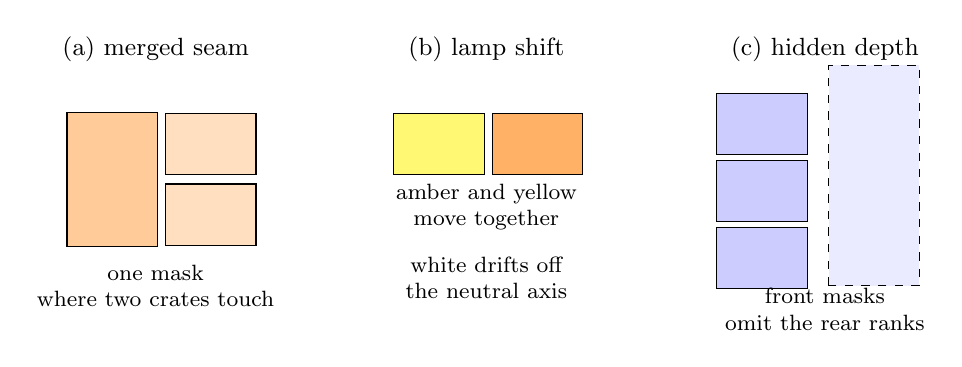
\begin{tikzpicture}[font=\footnotesize, cell/.style={draw, minimum width=1.15cm, minimum height=0.78cm, inner sep=0pt}]
  % panel A merged
  \begin{scope}[shift={(0,0)}]
    \node at (1.7,3.35) {\small (a) merged seam};
    \node[cell, fill=orange!40, minimum height=1.7cm] at (1.15,1.7) {};
    \node[cell, fill=orange!25] at (2.4,2.15) {};
    \node[cell, fill=orange!25] at (2.4,1.25) {};
    \node[align=center] at (1.7,0.35) {one mask\\where two crates touch};
  \end{scope}
  % panel B color
  \begin{scope}[shift={(4.6,0)}]
    \node at (1.3,3.35) {\small (b) lamp shift};
    \node[cell, fill=yellow!55] at (0.7,2.15) {};
    \node[cell, fill=orange!60] at (1.95,2.15) {};
    \node[align=center] at (1.3,1.35) {amber and yellow\\move together};
    \node[align=center] at (1.3,0.45) {white drifts off\\the neutral axis};
  \end{scope}
  % panel C depth
  \begin{scope}[shift={(8.7,0)}]
    \node at (1.5,3.35) {\small (c) hidden depth};
    \foreach \i in {0,1,2} {
      \node[cell, fill=blue!20] at (0.7,0.7+\i*0.85) {};
    }
    \draw[dashed, fill=blue!8] (1.55,0.35) rectangle (2.7,3.15);
    \node[align=center] at (1.5,0.05) {front masks\\omit the rear ranks};
  \end{scope}
\end{tikzpicture}
\caption{Three of the four failures that define the problem. A merged seam shortens the tally by a whole crate. A lamp shift confuses the pairs whose reflectances are nearest. Hidden depth is invisible to any mask model that sees only the side face. The fourth failure, a shadowed or clipped cell, is the one the lattice gap rule is drawn to fill.}
\label{fig:failures}
\end{figure}

\subsection{YOLO-vf-seg, and the two updates}
\label{sec:problem-gap}

YOLO-vf-seg is the baseline this thesis updates. It is a one-stage instance segmenter of the YOLOv8-seg type: a cross-stage backbone, a feature pyramid, a decoupled detection head, and a prototype mask assembly of the form~\eqref{eq:yolact}. The letters ``vf'' name a vertical-feature gate in the neck. On a side view the signal that separates stacked crates is a set of nearly horizontal lips, periodic in the vertical image coordinate. The gate pools each feature map along the horizontal axis, passes the resulting column through a small convolution, and multiplies the map by a sigmoid of that column, expanded back across the width. In equations, for a feature map $U\in\mathbb{R}^{C\times H\times W}$,
\begin{equation}
a = \sigma\!\left( g( \operatorname{GAP}_{w}(U) ) \right) \in (0,1)^{C\times H},
\qquad
\tilde{U}_{c,i,j} = a_{c,i}\, U_{c,i,j},
\label{eq:vf}
\end{equation}
where $\operatorname{GAP}_{w}$ is the mean over the width and $g$ is a $1\times 3$ convolution along the vertical axis followed by a pointwise map back to $C$ channels. This is coordinate attention restricted to the axis that carries the stack~\cite{hou2021coordatt}, placed in the neck rather than used as a generic module. It does not classify color and it does not count. It makes the lips easier for the mask head to see. The rest of the thesis treats YOLO-vf-seg as given, and does not claim it as a new architecture.

The updated system adds two modules, drawn in \Cref{fig:pipeline-overview}.

The illumination-invariant chromatic prototype head, ICPH, reads the pixels inside each mask and the mask-pooled features of the neck. It builds the eight-dimensional chromatic feature of Chapter~\ref{ch:methods}, standardizes it, and scores six color prototypes with a linear classifier. The head exists because of the second failure mode above. It is small enough that requirement~6 is not in doubt: the parameter count estimated in Chapter~\ref{ch:system} is under ten thousand weights on top of a medium segmenter.

Perspective lattice completion, PLC, reads the mask centers after they have been mapped by $H$ into metres on the front face. It estimates the origin of the lattice, snaps each center to an integer cell, fills a hole that has at least two orthogonal neighbors inside the bounding rectangle of the detections, and multiplies the number of occupied cells by the depth reading. The module exists because of the third and fourth failure modes. It is not a network, and it has no training iteration. Its only geometric parameters are the nominal pitch $(w,h)$, which \Cref{ass:lattice} fixes.

A third idea was considered and set aside. Training the segmenter with an auxiliary density loss, so that the integral of a density agrees with the number of masks, repairs inconsistency between two visible-count estimators. It does not see behind the front face, and it does not use the pitch. A fourth idea, a second camera above the pallet, would see the depth directly and would violate requirement~3. Both ideas remain available if the assumptions fail in a particular building. They are not the contributions.

The contributions are deliberately unequal in kind. ICPH is a learned head, and the estimate of it is an estimate of a classifier under a color model. PLC is a geometric algorithm, and the estimate of it is an estimate of a counter under a detection model. Putting them in one network and quoting a single average precision would hide the separate ways they fail. Chapter~\ref{ch:methods} derives each one. Chapter~\ref{ch:system} builds the passage system around both, and then estimates them separately under models that are written down in full.

\subsection{What is in scope, and how the thesis is organized}
\label{sec:scope}

The thesis is a system design and an estimate of that design. It specifies the camera's relation to the load, the segmenter, the color head, the lattice, the depth reading, and the way a passage is reduced to one answer. It does not report a field trial. The numbers in Chapter~\ref{ch:system} are produced by the Monte Carlo instrument \texttt{simulate\_estimation.py} under the observation model written there, with the seed fixed. They are estimates of the two modules. They are not accuracies measured on a brewery floor, and the text does not call them that.

Several related problems are named so that they are not silently included. Bottle-level inspection inside the crate, reading of printed lot codes, detection of a broken crate, and identity of the forklift are out of scope. So is any claim about a cardboard carton of unknown size. The lattice pitch is an input. If a second family of crates with a different pitch shares the aisle, the system needs a pitch hypothesis per family; that extension is described and not estimated.

The organization follows the three-chapter limit. This chapter has set out the principles, the prior systems, and the problem. \Cref{ch:methods} derives ICPH and then PLC, with the losses, the algorithms, and the complexity. \Cref{ch:system} specifies the passage system that holds the two modules, and then reports the estimate: protocol, tables, the worked passage, the parameter cost, and the limits of what the estimate can support.

The standard that the later chapters are written to is the standard of this problem statement. A module earns its place if it attacks one of the four failures in \Cref{fig:failures} or the invisible rank behind them, if it respects the side-view and timing requirements, and if its errors can be shown with a sign. ICPH and PLC are the two modules that meet that standard. The next chapter writes them down.
